%%%%%%%%%%%%%%%%%%%%%%%%%%%%%%%%%%%%%%%%%
% Beamer Presentation
% LaTeX Template
% Version 1.0 (10/11/12)
%
% This template has been downloaded from:
% http://www.LaTeXTemplates.com
%
% License:
% CC BY-NC-SA 3.0 (http://creativecommons.org/licenses/by-nc-sa/3.0/)
%
%%%%%%%%%%%%%%%%%%%%%%%%%%%%%%%%%%%%%%%%%

%----------------------------------------------------------------------------------------
%	PACKAGES AND THEMES
%----------------------------------------------------------------------------------------

\documentclass{beamer}

\mode<presentation> {

% The Beamer class comes with a number of default slide themes
% which change the colors and layouts of slides. Below this is a list
% of all the themes, uncomment each in turn to see what they look like.

%\usetheme{default}
%\usetheme{AnnArbor}
%\usetheme{Antibes}
%\usetheme{Bergen}
%\usetheme{Berkeley}
%\usetheme{Berlin}
%\usetheme{Boadilla}
%\usetheme{CambridgeUS}
%\usetheme{Copenhagen}
%\usetheme{Darmstadt}
%\usetheme{Dresden}
%\usetheme{Frankfurt}
%\usetheme{Goettingen}
%\usetheme{Hannover}
%\usetheme{Ilmenau}
%\usetheme{JuanLesPins}
%\usetheme{Luebeck}
\usetheme{Madrid}
%\usetheme{Malmoe}
%\usetheme{Marburg}
%\usetheme{Montpellier}
%\usetheme{PaloAlto}
%\usetheme{Pittsburgh}
%\usetheme{Rochester}
%\usetheme{Singapore}
%\usetheme{Szeged}
%\usetheme{Warsaw}

% As well as themes, the Beamer class has a number of color themes
% for any slide theme. Uncomment each of these in turn to see how it
% changes the colors of your current slide theme.

%\usecolortheme{albatross}
%\usecolortheme{beaver}
%\usecolortheme{beetle}
%\usecolortheme{crane}
%\usecolortheme{dolphin}
%\usecolortheme{dove}
%\usecolortheme{fly}
%\usecolortheme{lily}
%\usecolortheme{orchid}
%\usecolortheme{rose}
%\usecolortheme{seagull}
%\usecolortheme{seahorse}
%\usecolortheme{whale}
%\usecolortheme{wolverine}

%\setbeamertemplate{footline} % To remove the footer line in all slides uncomment this line
%\setbeamertemplate{footline}[page number] % To replace the footer line in all slides with a simple slide count uncomment this line

%\setbeamertemplate{navigation symbols}{} % To remove the navigation symbols from the bottom of all slides uncomment this line
}

\usepackage{graphicx} % Allows including images
\usepackage{booktabs} % Allows the use of \toprule, \midrule and \bottomrule in tables
\usepackage[utf8]{inputenc}

\setbeamertemplate{caption}{\raggedright\insertcaption\par}

\graphicspath{ {images/} }

%----------------------------------------------------------------------------------------
%	TITLE PAGE
%----------------------------------------------------------------------------------------

\title[BRKGA - BL - TOP]{Biased Random Key Genetic Algorithm con B\'usqueda Local para el Team Orienteering Problem} % The short title appears at the bottom of every slide, the full title is only on the title page

\author{Alejandro Lix Klett} % Your name
\institute[UBA] % Your institution as it will appear on the bottom of every slide, may be shorthand to save space
{
Directora: Prof. Dra. Irene Loiseau\\ 
\medskip
Departamento de Computaci\'on\\ % Your institution for the title page
%\textit{john@smith.com} % Your email address
}
\date{\today} % Date, can be changed to a custom date

\begin{document}

\begin{frame}
\titlepage % Print the title page as the first slide
\end{frame}

\begin{frame}
\frametitle{Contenido} % Table of contents slide, comment this block out to remove it
\tableofcontents % Throughout your presentation, if you choose to use \section{} and \subsection{} commands, these will automatically be printed on this slide as an overview of your presentation
\end{frame}

%----------------------------------------------------------------------------------------
%	PRESENTATION SLIDES
%----------------------------------------------------------------------------------------

%------------------------------------------------
\section{Orienteering Problem} % Sections can be created in order to organize your presentation into discrete blocks, all sections and subsections are automatically printed in the table of contents as an overview of the talk
%------------------------------------------------

%\subsection{Historia} % A subsection can be created just before a set of slides with a common theme to further break down your presentation into chunks
%\subsection{Descripci\'on}

\begin{frame}
\frametitle{Orienteering Problem}

\begin{itemize}
    \item Orientaci\'on es un deporte originario de Escandinavia
    \pause
    \item Cada jugador comienza en un punto de control y debe visitar tantos otros puntos de control como le sea posible dentro de un tiempo limite preespecificado. 
    \pause
    \item Cada punto de control tiene un puntaje.
    \pause
    \item Cada punto de control puede ser visitado una sola vez a lo sumo.
    \pause
    \item El objetivo es maximizar el puntaje total.
    \pause
    \item Este problema se conoce como Orienteering Problem (OP). El OP es NP-Hard como demostraron Golden, Levy y Vohra.
\end{itemize}

\end{frame}

%%%%%%%%%%%%%%%%%%%%%%%%%%%%%%%%%%%%%%%%%%%%%%

\section{Team Orienteering Problem}

\begin{frame}
\frametitle{Team Orienteering Problem}

\begin{itemize}
    \item Hay \textit{M} clientes, cada uno tiene un beneficio $b_i$ y una coordenada en el plano.
    \pause
    \item Los puntos de salida y llegada tienen beneficio cero
    \pause    
    \item Hay \textit{N} veh\'iculos
    \pause
    \item El beneficio de los clientes solo puede ser recolectado una vez.
    \pause
    \item El objetivo es maximizar la sumatoria de los beneficios recolectados de todos los vehículos.
    \pause
    \item Como TOP contiene a OP, es al menos tan dif\'icil.
\end{itemize}

\end{frame}

%%%%%%%%%%%%%%%%%%%%%%%%%%%%%%%%%%%%%%%%%%%%%%

\section{Ejemplo de solución de TOP}

\begin{frame}
\frametitle{Instancia p2.2.k del benchmark de Tsiligirides}

La instancia tiene dos vehículos con un $d_{max}$ = 22,50. Hay 19 clientes además de los puntos de salida y llegada.% La imagen muestra la solución óptima del problema.

\begin{figure}[h]
	\centering
	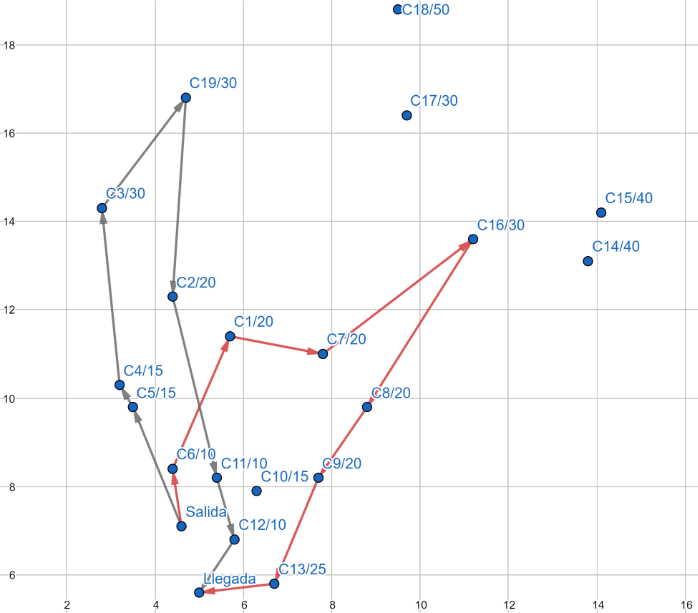
\includegraphics[width=7.5cm]{400cropped}
	\label{fig:400cropped}
\end{figure}


\end{frame}

%%%%%%%%%%%%%%%%%%%%%%%%%%%%%%%%%%%%%%%%%%%%%%

\section{Metaheurísticas}

\begin{frame}
\frametitle{Metaheurísticas}

\begin{itemize}
    \item Son métodos diseñados para encontrar buenas soluciones, en un tiempo razonable, a problemas de optimización combinatoria en general.
    \pause
    \item Las metaheurísticas son estrategias de alto nivel que guían una heurística específica del problema a resolver para mejorar su perfomance.
    \pause
\end{itemize}

Caracter\'isticas:

\begin{itemize}
    \item Son estrategias que gu\'ian procesos de búsqueda.
    \pause
    \item Sus conceptos se pueden describir con un gran nivel de abstracción. No son para un problema específico.
    \pause
    \item En muchos casos son algoritmos no-determin\'isticos.
    \pause
    \item Sus desarrollos y diseños suelen estar motivados por comportamientos naturales.
    \pause
    \item No garantizan que una soluci\'on \'optima sea encontrada.
    \pause
    \item Las t\'ecnicas metaheur\'isticas van desde algoritmos simples de b\'usqueda local a complejos procesos de aprendizaje.
\end{itemize}

\end{frame}

%%%%%%%%%%%%%%%%%%%%%%%%%%%%%%%%%%%%%%%%%%%%%%

\begin{frame}
\frametitle{Metaheurísticas}

Algunas técnicas:

\begin{itemize}
    \item Simulated Annealing
    \pause
    \item Tabu Search
    \pause
    \item Algoritmos evolutivos
    \pause
    \item Colonia de hormigas
    \pause
    \item Variable Neighborhood Search
    \pause
    \item Iterated Local Search
    \pause
    \item Etc
\end{itemize}

\end{frame}

%%%%%%%%%%%%%%%%%%%%%%%%%%%%%%%%%%%%%%%%%%%%%%

\section{Algoritmos Genéticos (GA)}

\begin{frame}
\frametitle{Algoritmos Genéticos (GA)}

\begin{itemize}
    \item Motivados en el concepto de supervivencia del más apto.
    \pause
    \item Los algoritmos genéticos manejan un conjunto de individuos.
    \pause
    \item Cada individuo es un cromosoma que codifica una solución.
    \pause
    \item Cada cromosoma tienen asociado un nivel de condición física que está correlacionado con el correspondiente valor de la función objetivo de la solución que codifica.
    \pause
    \item En cada generación se crea una nueva población con individuos provenientes de tres fuentes distintas: crossover, elites y mutantes.
\end{itemize}

\end{frame}

%%%%%%%%%%%%%%%%%%%%%%%%%%%%%%%%%%%%%%%%%%%%%%

\section{Random Key Genetic Algorithm (RKGA)}

\begin{frame}
\frametitle{Random Key Genetic Algorithm (RKGA)}

\begin{itemize}
    \item Los individuos son representados por un vector de números reales en el intervalo [0, 1].
    \pause
    \item La población inicial es generada al azar.
    \pause
    \item El decodificador es el responsable de convertir un cromosoma en una solución válida del problema.
    \pause
    \item En cada iteración se toman los mejores individuos y pasan directamente a la siguiente generación (elites).
    \pause
    \item La mayoría de los individuos de la nueva generación se genera cruzando dos individuos de la generación actual (crossover).
    \pause
    \item Un porcentaje muy bajo de los nuevos individuos es generado al azar, para escapar de mínimos locales (mutantes).
\end{itemize}

\end{frame}

%%%%%%%%%%%%%%%%%%%%%%%%%%%%%%%%%%%%%%%%%%%%%%

\section{Biased Random Key Genetic Algorithm (RKGA)}

\begin{frame}
\frametitle{Biased Random Key Genetic Algorithm (BRKGA)}

\begin{itemize}
    \item Cada individuo se genera combinando un elemento seleccionado al azar del conjunto de elite y el otro de la conjunto no-elite.
    \pause
    \item Parameterized Uniform Crossover. La probabilidad de que se trasmita el alelo del padre de elite es mayor que la del padre de no-elte.
    \pause
\end{itemize}

\end{frame}

%%%%%%%%%%%%%%%%%%%%%%%%%%%%%%%%%%%%%%%%%%%%%%

\begin{frame}
\frametitle{Diagrama de Flujo del BRKGA}

\begin{figure}[h]
	\centering
	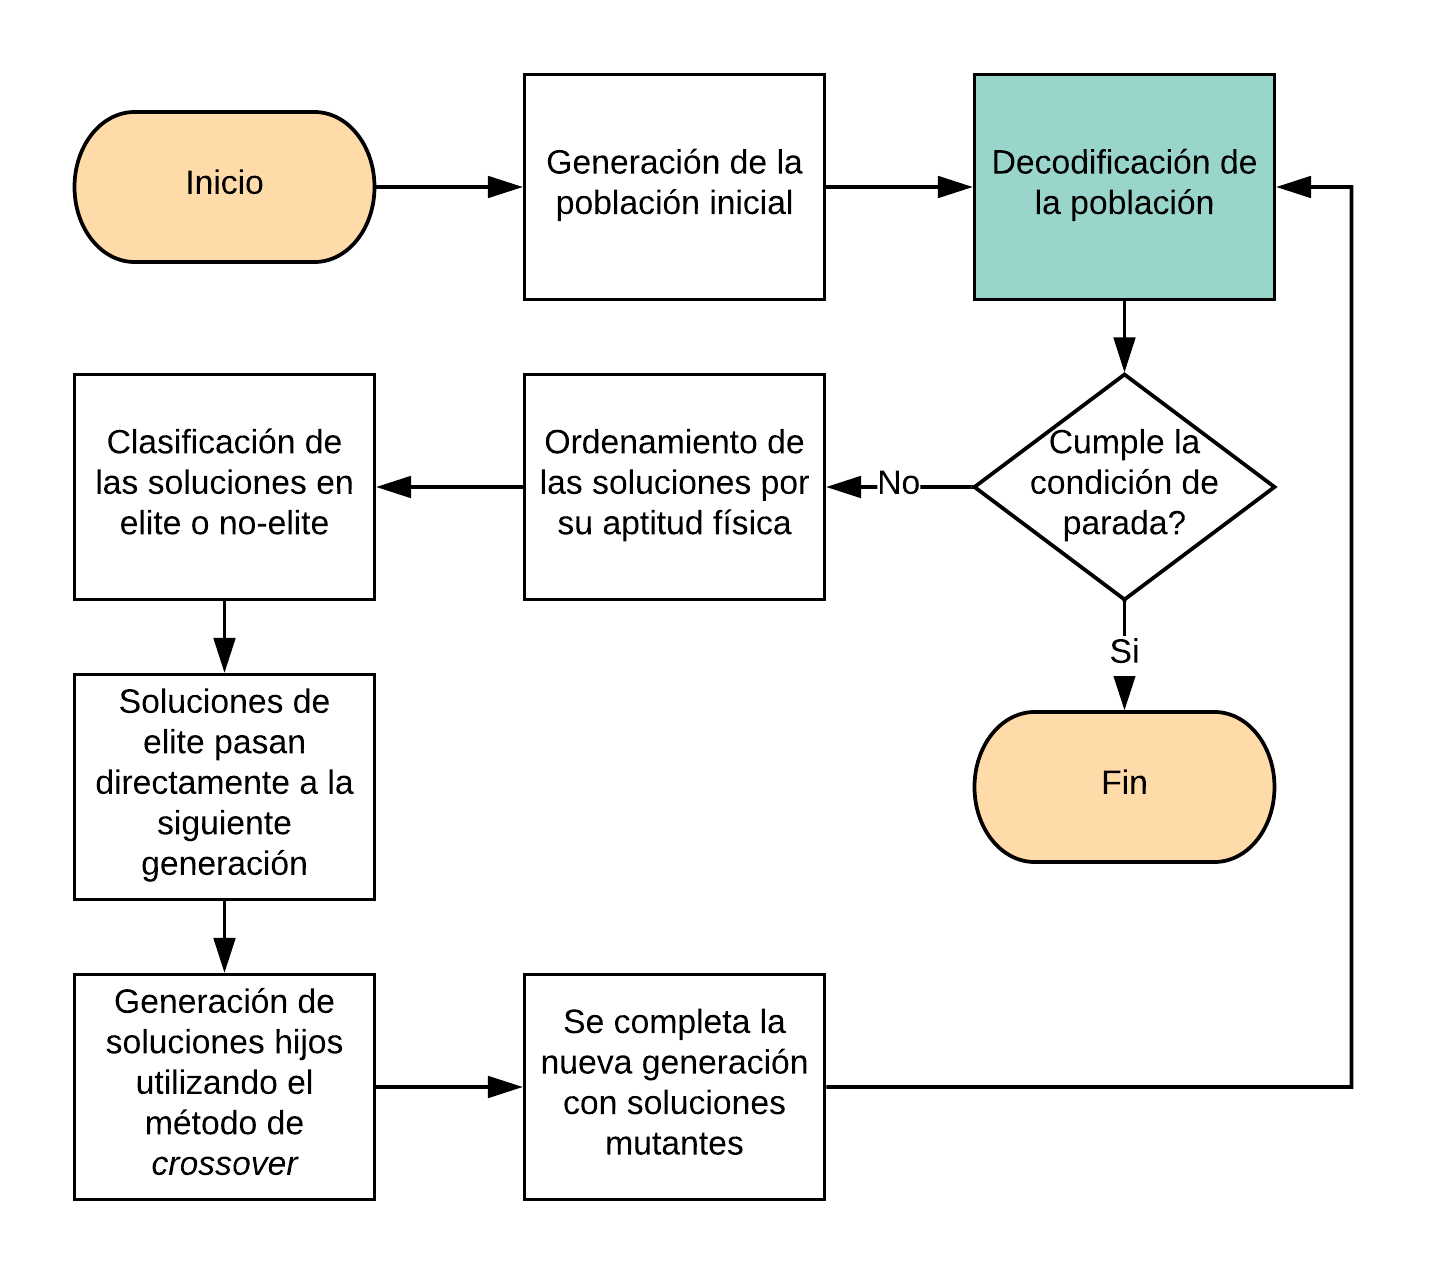
\includegraphics[width=8cm]{BRKGA_Flow_Chart_Base}
	\label{fig:BRKGA_Flow_Chart_Base}
\end{figure}

\end{frame}

%%%%%%%%%%%%%%%%%%%%%%%%%%%%%%%%%%%%%%%%%%%%%%

\begin{frame}
\frametitle{Generación de la Población Inicial}

\begin{itemize}
    \item Se crea una cantidad de vectores de enteros aleatorios igual a la cantidad de soluciones por generación que se desea.
    \pause
    \item Los vectores tienen un tamaño igual a la cantidad de clientes de la instancia.
    \pause
    \item Cada entero aleatorio del vector esta asociado a un identificador de cliente.
    \pause
\end{itemize}

\begin{figure}[h]
	\caption{Ejemplo de un nuevo vector de enteros aleatorios.}
	\centering
	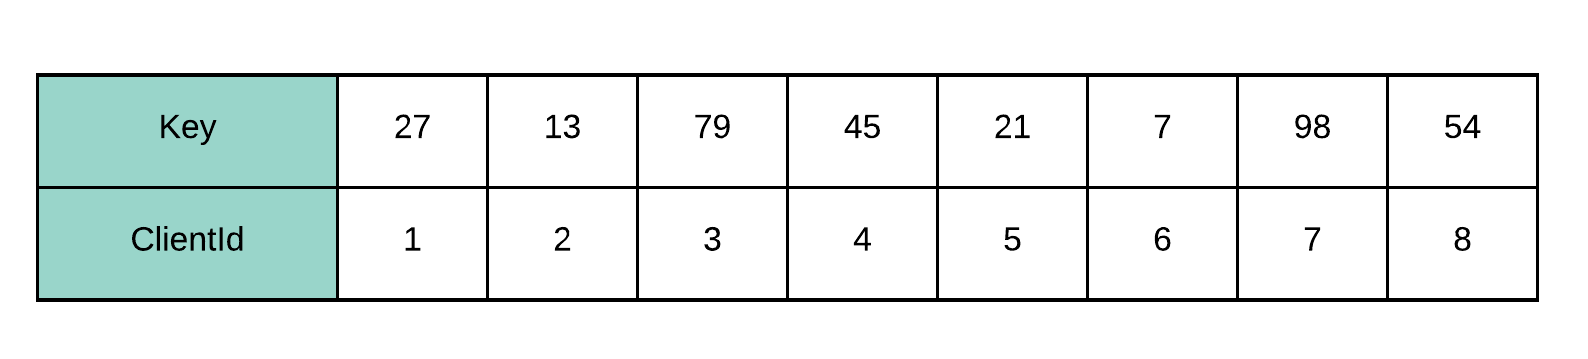
\includegraphics[width=9cm]{RandomKeysInicializado}
	\label{fig:RandomKeysInicializado}
\end{figure}

\end{frame}

%%%%%%%%%%%%%%%%%%%%%%%%%%%%%%%%%%%%%%%%%%%%%%

\begin{frame}
\frametitle{Decodificación de los vectores en soluciones validas del problema}

\begin{itemize}
    \item Se ordena el vector de enteros aleatorios por el valor de la clave aleatoria de forma ascendente.
    \pause
\end{itemize}

\begin{figure}[h]
	\caption{Ejemplo del vector de enteros aleatorios ordenado.}
	\centering
	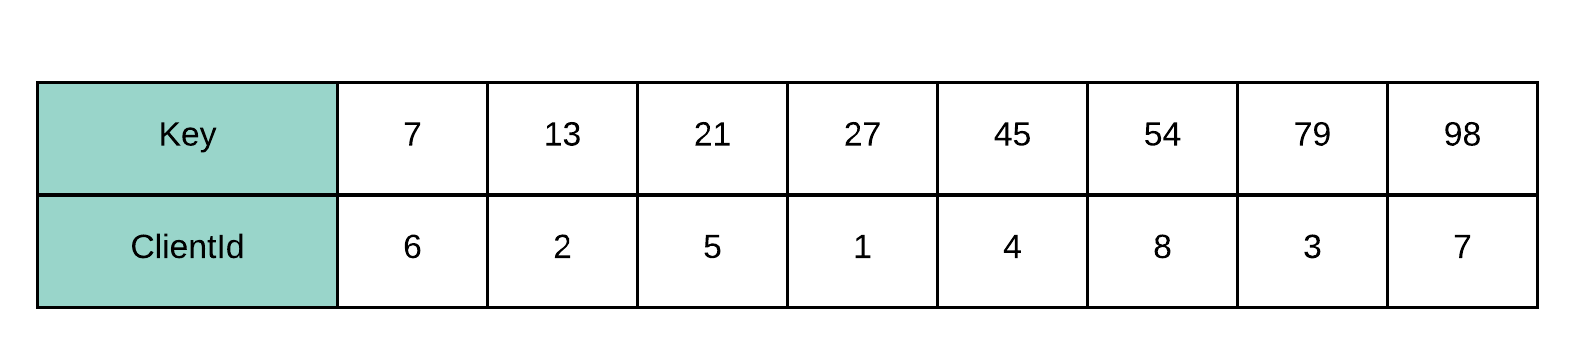
\includegraphics[width=9cm]{RandomKeysOrdenado}
	\label{fig:RandomKeysOrdenado}
\end{figure}

\begin{itemize}
    \pause
    \item Implementé dos decodificadores cada uno con su estrategia para generar soluciones.
    \pause
    \item Ambos decodificadores generan una solución válidas del problema a partir de un vector de enteros aleatorios ordenado.
\end{itemize}

\end{frame}

%%%%%%%%%%%%%%%%%%%%%%%%%%%%%%%%%%%%%%%%%%%%%%

\begin{frame}
\frametitle{Decodificador Simple}

\begin{itemize}
    \item Los vehículos están ordenados de forma ascendente según su identificador.
    \pause
    \item Toma el primer cliente e intenta agregarlo en la ruta del primer vehículo disponible.
    \pause
    \item Si logra insertarlo repite el proceso con el siguiente cliente para el mismo vehículo.
    \pause
    \item Si no lo logra, considera que la ruta del vehículo actual esta completa e intenta agregar el mismo cliente en el siguiente vehículo disponible.
    \pause
    \item Repite hasta completar la ruta de todos los vehículos disponibles.
    \pause
\end{itemize}

\begin{figure}[h]
	\caption{Ejemplo de la solución generada por el decodificador simple}
	\centering
	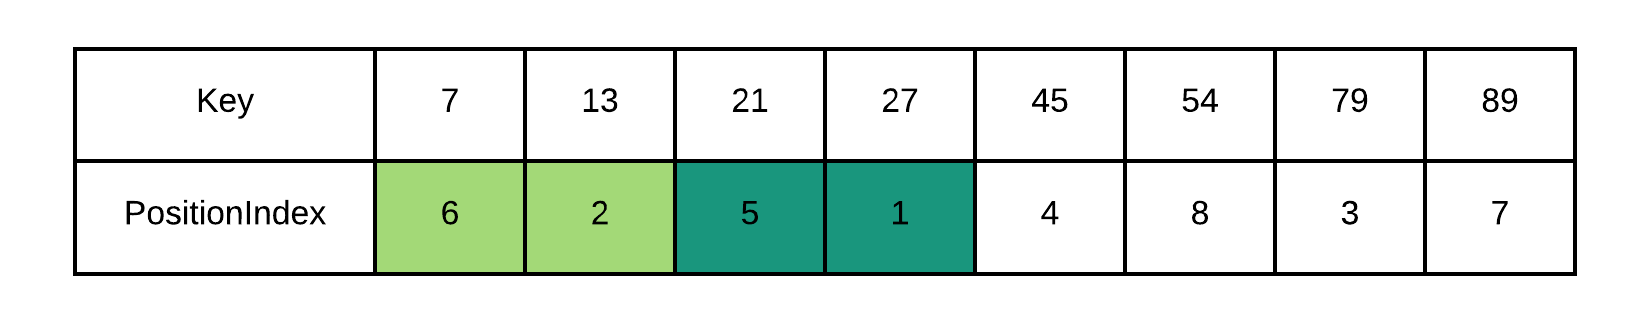
\includegraphics[width=9cm]{DistribucionClientesDecoSimple}
	\label{fig:DistribucionClientesDecoSimple}
\end{figure}

\end{frame}

%%%%%%%%%%%%%%%%%%%%%%%%%%%%%%%%%%%%%%%%%%%%%%

\begin{frame}
\frametitle{Decodificador Goloso}

\begin{itemize}
    \item Se diferencia del decodificador simple en el momento en que encuentra un cliente que no entra en la ruta del vehículo actual.
    \pause
    \item En vez de pasar al siguiente vehículo, prueba con el siguiente cliente.
    \pause
    \item Por lo tanto por cada vehículo prueba todos los clientes en el orden dado.
    \pause
    \item No prueba con los clientes que ya fueron asignados a otro vehículo
    \pause
\end{itemize}

\begin{figure}[h]
	\caption{Ejemplo de la solución generada por el decodificador goloso}
	\centering
	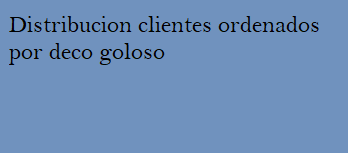
\includegraphics[width=9cm]{DistribucionClientesDecoGoloso}
	\label{fig:DistribucionClientesDecoGoloso}
\end{figure}

\end{frame}

%%%%%%%%%%%%%%%%%%%%%%%%%%%%%%%%%%%%%%%%%%%%%%

\begin{frame}
\frametitle{Comparación entre Decodificadores}

\begin{itemize}
    \item Se realizó una prueba para comparar los tiempos de ejecución y aptitud de las soluciones generadas por ambos decodificadores.
    \pause
    \item Se crearon 200 vectores de enteros aleatorios y se decodificaron utilizando ambos decodificadores.
    \pause
\end{itemize}

\begin{figure}[h]
	\caption{Ejemplo de la solución generada por el decodificador goloso}
	\centering
	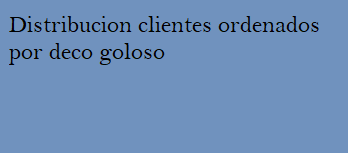
\includegraphics[width=9cm]{DistribucionClientesDecoGoloso}
	\label{fig:DistribucionClientesDecoGoloso}
\end{figure}

\end{frame}

%%%%%%%%%%%%%%%%%%%%%%%%%%%%%%%%%%%%%%%%%%%%%%

\begin{frame}
\frametitle{Biased Crossover}

\begin{figure}[h]
	\centering
	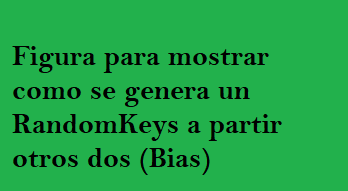
\includegraphics[width=8cm]{BiasCrossover}
	\label{fig:BiasCrossover}
\end{figure}

\end{frame}

%%%%%%%%%%%%%%%%%%%%%%%%%%%%%%%%%%%%%%%%%%%%%%

\begin{frame}
\frametitle{Evolución de la Población}

\begin{figure}[h]
	\centering
	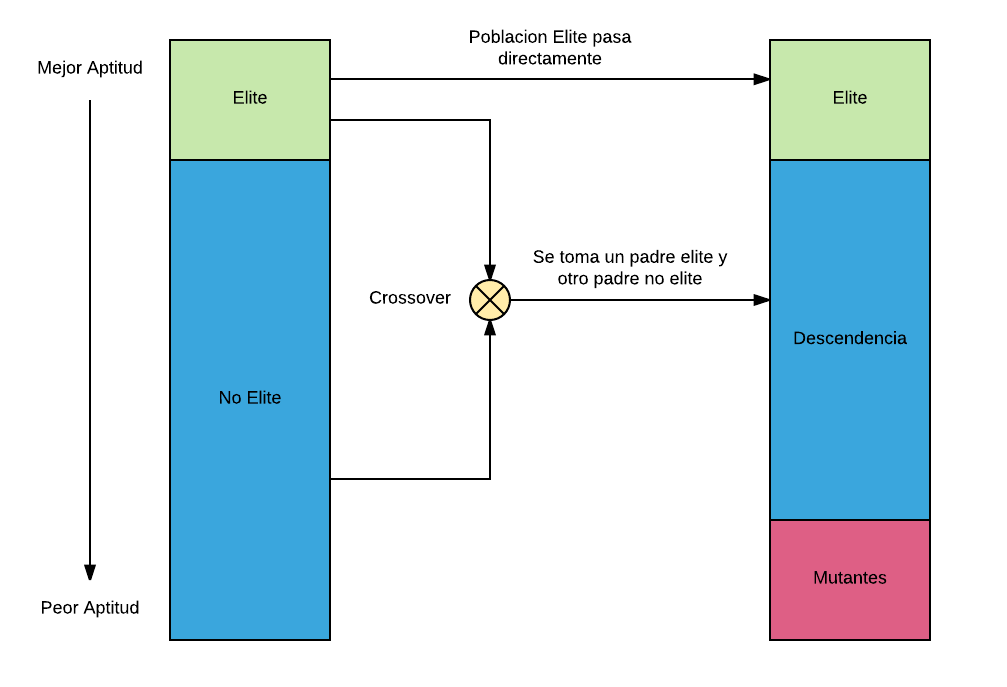
\includegraphics[width=10cm]{EvolucionPoblacion}
	\label{fig:EvolucionPoblacion}
\end{figure}

\end{frame}

%%%%%%%%%%%%%%%%%%%%%%%%%%%%%%%%%%%%%%%%%%%%%%

\begin{frame}
\frametitle{Flow Chart del BRKGA con Búsqueda Local}

\begin{figure}[h]
	\centering
	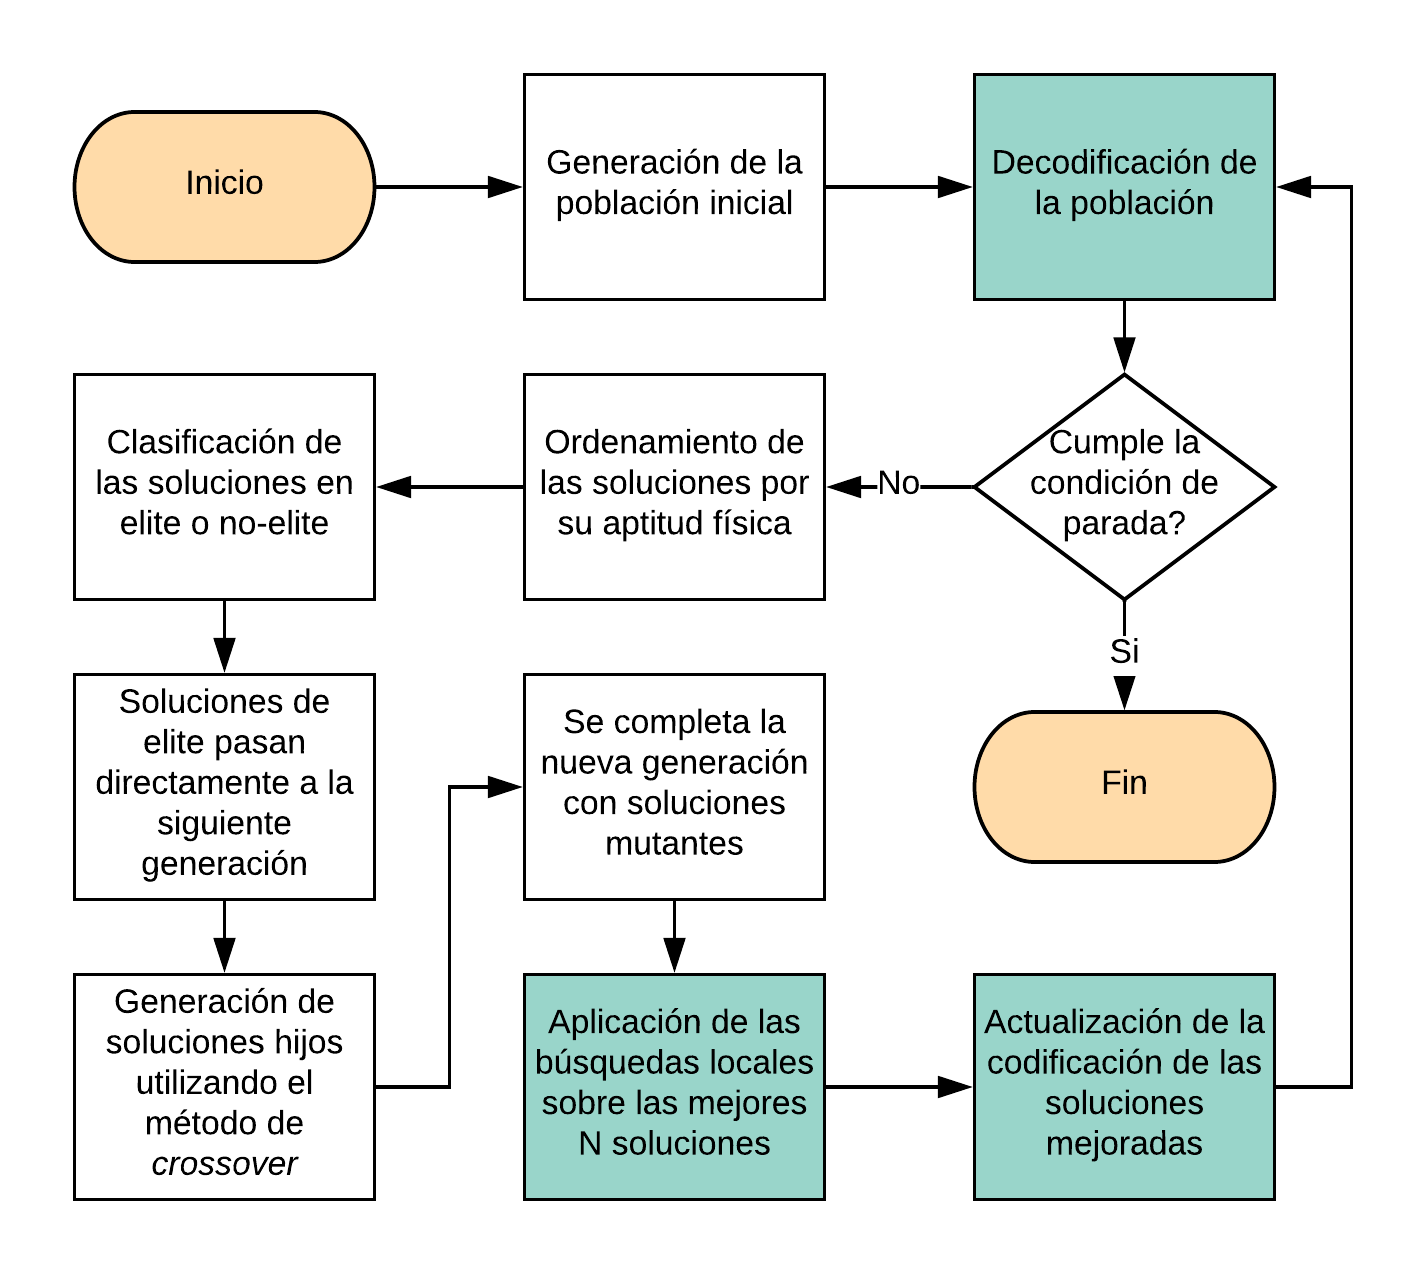
\includegraphics[width=8cm]{BRKGA_Flow_Chart_Implementado}
	\label{fig:BRKGA_Flow_Chart_Implementado}
\end{figure}

\end{frame}

%%%%%%%%%%%%%%%%%%%%%%%%%%%%%%%%%%%%%%%%%%%%%%

\begin{frame}
\frametitle{Flow Chart del BRKGA con Búsqueda Local}

\begin{itemize}
    \item 
    \pause
    \item 
    \pause
    \item 
    \pause
    \item 
    \pause
    \item 
    \pause
\end{itemize}

\end{frame}

%%%%%%%%%%%%%%%%%%%%%%%%%%%%%%%%%%%%%%%%%%%%%%

\begin{frame}
\frametitle{Flow Chart del BRKGA con Búsqueda Local}

\begin{itemize}
    \item 
    \pause
    \item 
    \pause
    \item 
    \pause
    \item 
    \pause
    \item 
    \pause
\end{itemize}

\end{frame}

%%%%%%%%%%%%%%%%%%%%%%%%%% EJEMPLOS %%%%%%%%%%%%%%%%

\begin{frame}

\frametitle{Paragraphs of Text}
Sed iaculis dapibus gravida. Morbi sed tortor erat, nec interdum arcu. Sed id lorem lectus. Quisque viverra augue id sem ornare non aliquam nibh tristique. Aenean in ligula nisl. Nulla sed tellus ipsum. Donec vestibulum ligula non lorem vulputate fermentum accumsan neque mollis.\\~\\

Sed diam enim, sagittis nec condimentum sit amet, ullamcorper sit amet libero. Aliquam vel dui orci, a porta odio. Nullam id suscipit ipsum. Aenean lobortis commodo sem, ut commodo leo gravida vitae. Pellentesque vehicula ante iaculis arcu pretium rutrum eget sit amet purus. Integer ornare nulla quis neque ultrices lobortis. Vestibulum ultrices tincidunt libero, quis commodo erat ullamcorper id.
\end{frame}

%------------------------------------------------

\begin{frame}
\frametitle{Bullet Points}
\begin{itemize}
\item Lorem ipsum dolor sit amet, consectetur adipiscing elit
\item Aliquam blandit faucibus nisi, sit amet dapibus enim tempus eu
\item Nulla commodo, erat quis gravida posuere, elit lacus lobortis est, quis porttitor odio mauris at libero
\item Nam cursus est eget velit posuere pellentesque
\item Vestibulum faucibus velit a augue condimentum quis convallis nulla gravida
\end{itemize}
\end{frame}

%------------------------------------------------

\begin{frame}
\frametitle{Blocks of Highlighted Text}
\begin{block}{Block 1}
Lorem ipsum dolor sit amet, consectetur adipiscing elit. Integer lectus nisl, ultricies in feugiat rutrum, porttitor sit amet augue. Aliquam ut tortor mauris. Sed volutpat ante purus, quis accumsan dolor.
\end{block}

\begin{block}{Block 2}
Pellentesque sed tellus purus. Class aptent taciti sociosqu ad litora torquent per conubia nostra, per inceptos himenaeos. Vestibulum quis magna at risus dictum tempor eu vitae velit.
\end{block}

\begin{block}{Block 3}
Suspendisse tincidunt sagittis gravida. Curabitur condimentum, enim sed venenatis rutrum, ipsum neque consectetur orci, sed blandit justo nisi ac lacus.
\end{block}
\end{frame}

%------------------------------------------------

\begin{frame}
\frametitle{Multiple Columns}
\begin{columns}[c] % The "c" option specifies centered vertical alignment while the "t" option is used for top vertical alignment

\column{.45\textwidth} % Left column and width
\textbf{Heading}
\begin{enumerate}
\item Statement
\item Explanation
\item Example
\end{enumerate}

\column{.5\textwidth} % Right column and width
Lorem ipsum dolor sit amet, consectetur adipiscing elit. Integer lectus nisl, ultricies in feugiat rutrum, porttitor sit amet augue. Aliquam ut tortor mauris. Sed volutpat ante purus, quis accumsan dolor.

\end{columns}
\end{frame}

%------------------------------------------------
\section{Second Section}
%------------------------------------------------

\begin{frame}
\frametitle{Table}
\begin{table}
\begin{tabular}{l l l}
\toprule
\textbf{Treatments} & \textbf{Response 1} & \textbf{Response 2}\\
\midrule
Treatment 1 & 0.0003262 & 0.562 \\
Treatment 2 & 0.0015681 & 0.910 \\
Treatment 3 & 0.0009271 & 0.296 \\
\bottomrule
\end{tabular}
\caption{Table caption}
\end{table}
\end{frame}

%------------------------------------------------

\begin{frame}
\frametitle{Theorem}
\begin{theorem}[Mass--energy equivalence]
$E = mc^2$
\end{theorem}
\end{frame}

%------------------------------------------------

\begin{frame}[fragile] % Need to use the fragile option when verbatim is used in the slide
\frametitle{Verbatim}
\begin{example}[Theorem Slide Code]
\begin{verbatim}
\begin{frame}
\frametitle{Theorem}
\begin{theorem}[Mass--energy equivalence]
$E = mc^2$
\end{theorem}
\end{frame}\end{verbatim}
\end{example}
\end{frame}

%------------------------------------------------

\begin{frame}
\frametitle{Figure}
Uncomment the code on this slide to include your own image from the same directory as the template .TeX file.
%\begin{figure}
%\includegraphics[width=0.8\linewidth]{test}
%\end{figure}
\end{frame}

%------------------------------------------------

\begin{frame}[fragile] % Need to use the fragile option when verbatim is used in the slide
\frametitle{Citation}
An example of the \verb|\cite| command to cite within the presentation:\\~

This statement requires citation \cite{p1}.
\end{frame}

%------------------------------------------------

\begin{frame}
\frametitle{References}
\footnotesize{
\begin{thebibliography}{99} % Beamer does not support BibTeX so references must be inserted manually as below
\bibitem[Smith, 2012]{p1} John Smith (2012)
\newblock Title of the publication
\newblock \emph{Journal Name} 12(3), 45 -- 678.
\end{thebibliography}
}
\end{frame}

%------------------------------------------------

\begin{frame}
\Huge{\centerline{The End}}
\end{frame}

%----------------------------------------------------------------------------------------

\end{document} 